\section{Análise da Arquitetura do Now in Android}\label{sec:arquitetura}
\subsection{Camadas e Padrões}
A documentação descreve UI, Domain e Data, com eventos encaminhados para
operações e dados observados por Flow~\cite{nia-arquitetura}. O domínio é
opcional nas recomendações Android: encapsula regras complexas ou
reutilizadas, e pode depender da camada de dados~\cite{android-dominio}.
A Figura~\ref{fig:camadas} distingue dependências e observação de dados.

Na UI, Compose apresenta estado e encaminha ações. O ViewModel mantém
\texttt{State\allowbreak Flow} e executa operações no seu escopo. Essa organização é
compatível com MVVM, mas MVVM descreve a apresentação, não todas as decisões
do sistema. UDF descreve a direção das interações, sem exigir ligação
bidirecional entre propriedades visuais e dados.

\begin{figure*}[t]
\centering
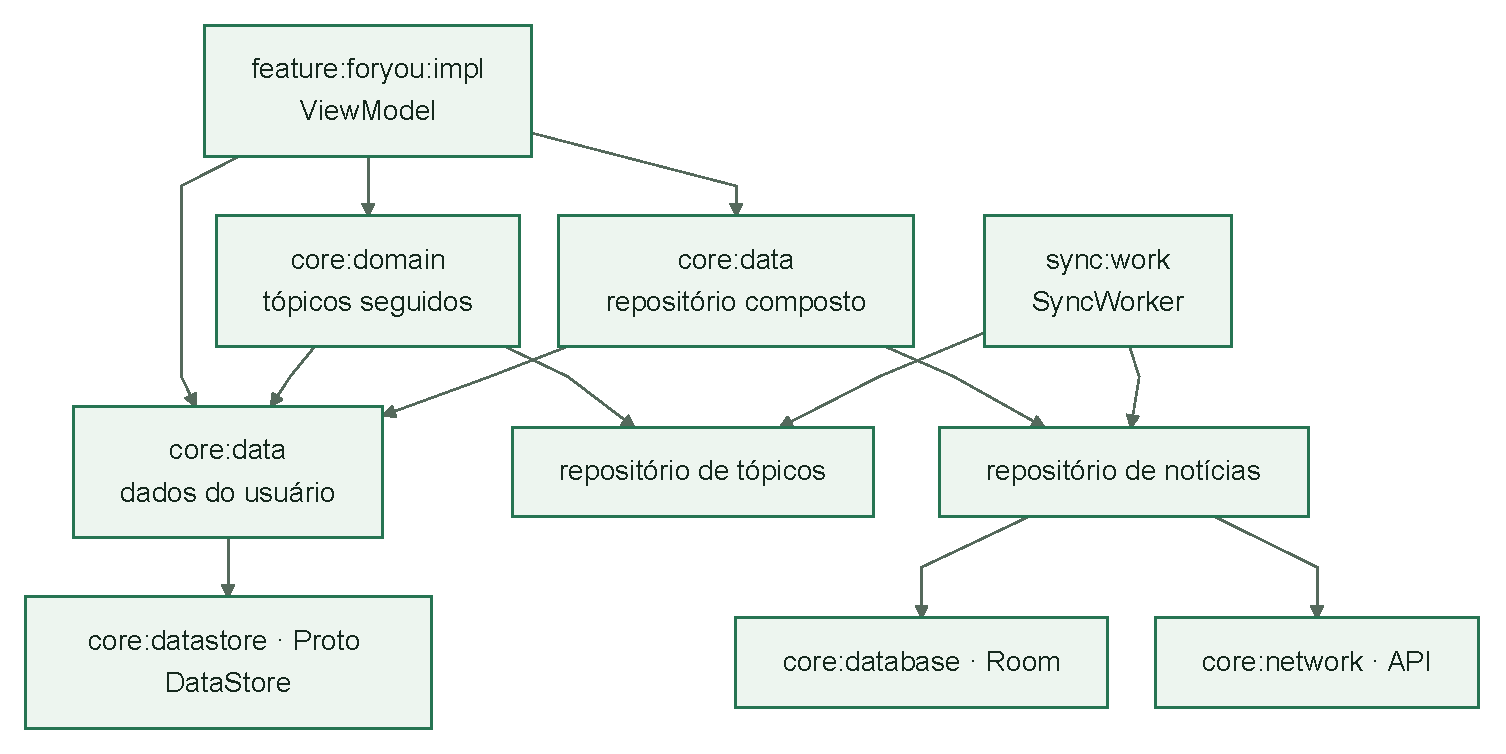
\includegraphics[width=\textwidth]{imagens/02-componentes.pdf}
\caption{Componentes do recorte For You e sincronização. Rótulos curtos
representam repositórios e módulos; não são um inventário completo do sistema.}
\Description{For You usa domínio, repositório composto e dados do usuário. O composto depende de notícias e usuário, apoiados em Room, rede e DataStore. SyncWorker coordena notícias e tópicos.}
\label{fig:componentes}
\end{figure*}

\begin{figure*}[t]
\centering
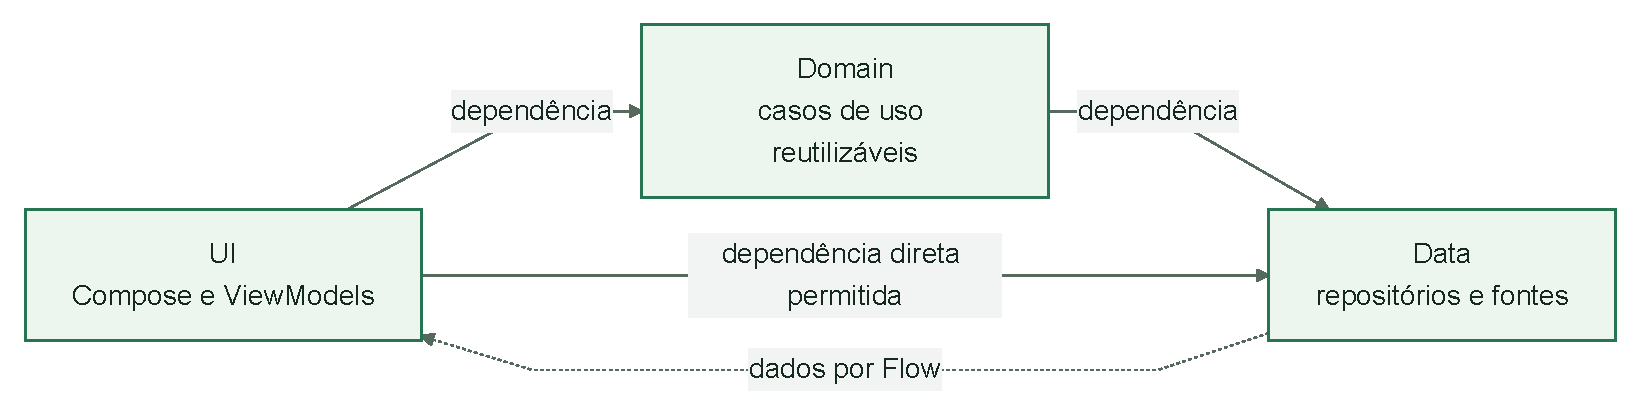
\includegraphics[width=\textwidth]{imagens/03-camadas.pdf}
\caption{Camadas do NiA. Setas contínuas indicam dependências de código;
a tracejada representa observação reativa. A UI pode usar dados diretamente.}
\Description{UI depende de Domain e Data. Domain depende de Data. Dados observáveis retornam à UI por Flow.}
\label{fig:camadas}
\end{figure*}

Na camada de dados, interfaces como \texttt{News\allowbreak Repository} e
\texttt{User\allowbreak Data\allowbreak Repository} ocultam fontes. O
\texttt{Composite\allowbreak User\allowbreak News\allowbreak Resource\allowbreak Repository} associa notícias a preferências.
Esse encapsulamento favorece substituição, mas acrescenta contratos e
coordenação de fluxos. A modularização da Figura~\ref{fig:componentes} explicita
limites; seu custo inclui configuração e evolução das dependências.

Hilt vincula interfaces a implementações em \texttt{Data\allowbreak Module} e injeta o
ViewModel; na revisão atual há também injeção assistida para a chave de
navegação. Isso reduz montagem manual, mas introduz geração de código e
configuração. O uso de Flow permite recomposição a partir de mudanças,
exigindo atenção a cancelamento, assinaturas e concorrência.

\subsection{Persistência, Sincronização e For You}
O repositório \texttt{Offline\allowbreak First\allowbreak News\allowbreak Repository} consulta Room e
sincroniza atualizações remotas.

Preferências e favoritos ficam no Proto DataStore,
acessado por \texttt{Nia\allowbreak Preferences\allowbreak Data\allowbreak Source}. WorkManager executa \texttt{Sync\allowbreak Worker}. A disponibilidade local tem como contrapartida a
possibilidade de conteúdo desatualizado e o custo de sincronização, coerente
com a orientação offline-first~\cite{android-offline}.

O feed de For You chama
\texttt{observe\allowbreak All\allowbreak For\allowbreak Followed\allowbreak Topics()} no repositório composto. Ele observa os
tópicos seguidos e combina notícias com dados do usuário; o ViewModel converte
a emissão em \texttt{News\allowbreak Feed\allowbreak Ui\allowbreak State.Success}, inicialmente \texttt{Loading}.
Para salvar, a ação \texttt{update\allowbreak News\allowbreak Resource\allowbreak Saved} delega a gravação.
O método chamado é \texttt{set\allowbreak News\allowbreak Resource\allowbreak Bookmarked}. DataStore emite a alteração e o feed é
recalculado. O domínio permanece exemplificado pelo
\texttt{Get\allowbreak Followable\allowbreak Topics\allowbreak Use\allowbreak Case}, usado no onboarding.

Há uma divergência relevante: a jornada ainda cita
\texttt{Get\allowbreak User\allowbreak News\allowbreak Resources\allowbreak Use\allowbreak Case}, ausente na árvore estudada. Por isso,
a sequência usa os participantes do código atual. A organização em camadas
não constitui evidência de adesão integral a Clean Architecture ou Arquitetura
Hexagonal; essas classificações exigiriam verificar suas regras específicas.
